\newcommand{\templatesdir}{../../../templates}
\newcommand{\template}{template-material}
\input{\templatesdir/\template/template}

\newcommand{\initials}{45EST}
\newcommand{\discipline}{Algoritmos e Estruturas de Dados}
\newcommand{\doctitle}{Guia para os exercícios}
\newcommand{\myname}{Prof. Marcelo de Souza}
\newcommand{\university}{Universidade do Estado de Santa Catarina}
\newcommand{\campus}{Centro de Educação Superior do Alto Vale do Itajaí}
\newcommand{\department}{Departamento de Engenharia de Software}
\newcommand{\exercisedescription}{Exercício}

\usepackage{listings}
\lstset{language=Java,
	showspaces=false,
	showtabs=false,
	breaklines=true,
	showstringspaces=false,
	breakatwhitespace=true,
	commentstyle=\color{green!60!black},
	keywordstyle=\color{blue},
	stringstyle=\color{orange!80!black},
	basicstyle=\ttfamily,
	numberstyle=\tiny\color{gray},
	tabsize=3
}

\setlength{\parskip}{0.3em}

\begin{document}
	
\inserttitle

\textbf{Importante:} as informações apresentadas neste documento visam conduzir o estudante na resolução dos exercícios da disciplina. Na maioria dos casos, são apresentados apenas os direcionamentos da solução esperada. Cabe ao estudante o desenvolvimento completo da solução.

\section{Introdução}

\paragraph{Exercício 1:}
O jogo deve ser implementado utilizando a estrutura de dados baseada em matriz. Para medir a memória utilizada, os métodos utilitários de \texttt{Runtime} podem ser aplicados. Para medir o tempo de processamento, deve-se medir a diferença dos timestamps antes e depois da execução.

\paragraph{Exercício 2:}
Uma primeira tentativa consiste em armazenar apenas as posições onde existem elementos. Para isso, crie uma classe com o tipo de elemento e a coordenada que representa sua posição. Todas as operações podem ser realizadas utilizando essa nova estrutura, com menor consumo de memória e tempo de processamento.

\section{Complexidade de algoritmos}

\paragraph{Exercício 1:}
Exercício de leitura.

\paragraph{Exercício 2:}
Exercício de leitura.

\paragraph{Exercício 3:}
Leia a Seção 3.5.2 de~\cite{GoodrichAndTamassia2013}.

\paragraph{Exercício R-4.1:}
Uma dica é utilizar potências de dois como seu valor para $n$.

\paragraph{Exercício R-4.2:}
Ao igualar as duas equações e simplificá-las, vemos que o cruzamento ocorre em $n = 4 \log n$. Agora, podemos confirmar que o cruzamento ocorre em $n = 2^4 = 16$.

\paragraph{Exercício R-4.3:}
Ao igualar as duas equações e simplificá-las temos a confirmação de que o cruzamento ocorre em $n = 20$. Ou seja, $40 n^2 \le 2n^3$ para $n \ge 20$.

\paragraph{Exercício R-4.8:}
Simplifique as expressões e então use o ordenamento das funções estudadas em sala de aula para ordenar o conjunto. Resultado: $2^{10}$, $2^{\log n}$, $3n + 100 \log n$, $4n$, $n \log n$, $4n \log n + 2n$, $n^2 + 10n$, $n^3$, $2^n$.

\paragraph{Exercício R-4.9:}
Considere o número de vezes que o laço é executado e quantas operações primitivas ocorrem em cada iteração. O algoritmo executa em tempo $O(n)$.

\paragraph{Exercício R-4.10:}
Considere o número de vezes que o laço é executado e quantas operações primitivas ocorrem em cada iteração. O algoritmo executa em tempo $O(n)$.

\paragraph{Exercício R-4.11:}
Considere o número de vezes que o laço interno é executado e quantas operações primitivas ocorrem em cada iteração, e então faça o mesmo para o laço externo. O algoritmo executa em tempo $O(n^2)$.

\paragraph{Exercício R-4.12:}
Considere o número de vezes que o laço interno é executado e quantas operações primitivas ocorrem em cada iteração, e então faça o mesmo para o laço externo. O algoritmo executa em tempo $O(n)$.

\paragraph{Exercício R-4.13:}
Considere o número de vezes que o laço interno é executado e quantas operações primitivas ocorrem em cada iteração, e então faça o mesmo para os dois laços externos. O algoritmo executa em tempo $O(n^3)$.

\paragraph{Exercício R-4.28:}
Os números na primeira linha são bastante grandes. A tabela abaixo calcula os valores de maneira aproximada em potência de 10. Valores aproximados são suficientes para verificar a ordem de grandeza em termos de complexidade.

\begin{figure}[H]
	\centering
	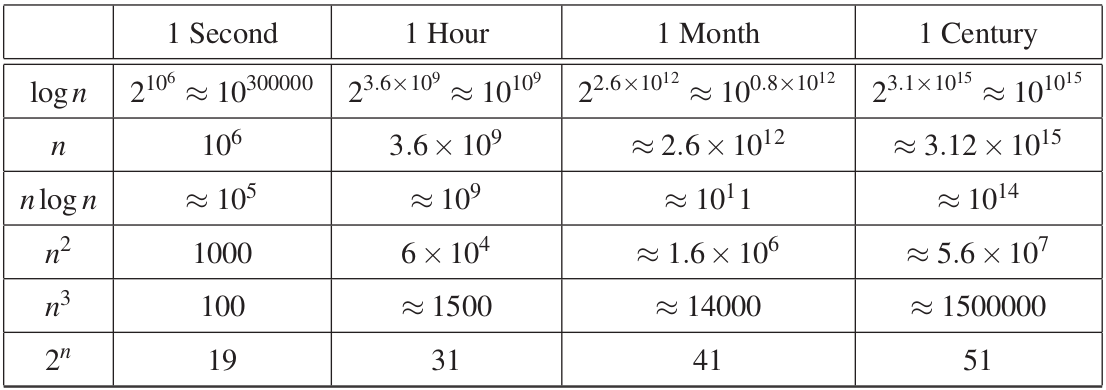
\includegraphics[width=0.7\linewidth]{img/r-4-28}
\end{figure}

\paragraph{Exercício R-4.29:}
$O(n \log n)$.

\paragraph{Exercício R-4.30:}
$O(n \log n)$.

\paragraph{Exercício R-4.31:}
$O(n^2)$ (quando todos os elementos são pares).

\paragraph{Exercício R-4.32:}
Tempo de execução é proporcional a $\sum_{i = 1}^{n} i = O(n^2)$.

\paragraph{Exercício R-4.34:}
Veja a discussão sobre número Harmônico em~\cite{GoodrichEtAl2014}.

\paragraph{Exercício P-4.60:}
Exercício de implementação (escolha valores representativos da entrada do tamanho $n$ e faça pelo menos $5$ testes para cada valor de tamanho $n$).

\paragraph{Exercício P-4.61:}
Exercício de implementação.

\paragraph{Exercício P-4.62:}
Exercício de implementação (você deverá tentar executar a operação várias vezes para muitos problemas de tamanhos diferentes).

\paragraph{Exercício P-4.63:}
Exercício de implementação.


\section{Estruturas de dados fundamentais}

\paragraph{Exercício 1:}
Exercício de leitura.

\paragraph{Exercício R-3.5:}
Modifique o código e teste as alterações. Não há consequências negativas em remover aquelas linhas (na verdade deverá ter um leve aumento na eficiência). Enquanto o estado interno parece estar inconsistente com o \texttt{tail} referenciando um nó ``inexistente'', a referência \texttt{tail} nunca é acessada em uma lista vazia, então a inconsistência não tem efeito.

\paragraph{Exercício R-3.6:}
Uma possível solução consiste em um algoritmo linear simples.

\begin{lstlisting}[frame=single]
private Node<E> penultimate(){
	if(size<2)
		throw new IllegalStateExeception("list must have 2 or more entries");
	Node<E> walk = head;
	while(walk->next->next != null)
		walk = walk->next;
	return walk;
}
\end{lstlisting}

\paragraph{Exercício R-3.7:}
Existe uma solução de linha única.

\begin{lstlisting}[frame=single]
tail.setNext(new Node<>(e, tail.getNext()))
\end{lstlisting}

\paragraph{Exercício R-3.8:}
Considere uma busca combinada de ambas extremidades. Também, lembrar que um \textit{link hop} é uma atribuição do formato \texttt{p = p.getNext();} ou \texttt{p = p.getPrev();}. O método a seguir roda no tempo $O(n)$.

\begin{lstlisting}[frame=single]
private Node<E> middle(){
	if(size == 0)
		throw new IllegalStateException("list must be nonempty");
	Node<E> moddle = header->next
	Node<E> partner = trailer->prev;
	while(middle != partner && middle->next != partner){
		middle = middle.getNext();
		partner = partner.getPrev();
	}
	return middle;
}
\end{lstlisting}

\paragraph{Exercício R-3.9:}
Use um laço para percorrer a lista enquanto conta.

\begin{lstlisting}[frame=single]
public int size(){
	int count = 0;
	Node<E> walk = head;
	while(walk != null){
		count++;
		walk = walk.getNext();
	}
	return count;
}
\end{lstlisting}

\paragraph{Exercício R-3.10:}
Você precisa acompanhar onde você começou ou seu método fará um laço infinito.

\begin{lstlisting}[frame=single]
public int size(){
	if(tail == null)
		return 0;
	Node<E> wal = tail->next;
	int count = 1;
	while(walk != tail){
		count++;
		walk = walk.getNext();
	}
	return count;
}
\end{lstlisting}

\paragraph{Exercício R-3.11:}
Não inclua o sentinela na contagem.

\begin{lstlisting}[frame=single]
public int size(){
	int count = 0;
	Node<E> walk = header->next;
	while(walk != trailer){
		count++;
		walk = walk.getNext();
	}
	return count;
}
\end{lstlisting}

\paragraph{Exercício R-3.15:}
Como sugestão, você pode contar com a variável tamanho para correr o número de passos corretos quando percorrer a lista.

\paragraph{Exercício R-3.16:}
Como sugestão, considere que os sentinelas são irrelevantes à equivalência de duas listas.

\paragraph{Exercício C-3.25:}
A operação de concatenação não precisa procurar tudo em $L$ e $M$. Use um nodo temporário para caminhar até o final da lista $L$. Então, faça o último elemento de $L$ apontar para o primeiro elemento de $M$ como seu próximo nodo. O número de passos é proporcional ao tamanho de $L$.

\begin{lstlisting}[frame=single,language=Pascal]
Concatenate(L,M)
	Create a node v
	v = L.getHead()
	while v.getNext() != null do
		v = v.getNext()
	v.setNext(M.getHead())
	return L
\end{lstlisting}

\paragraph{Exercício C-3.26:}
Junte o final de $L$ no começo de $M$. Use dois nodos temporários, \texttt{temp1} e \texttt{temp2}. Inicialize \texttt{temp1} como o \texttt{trailer} de $L$ e \texttt{temp2} como o \texttt{header} de $M$. Atribua \texttt{temp2} como o próximo elemento de \texttt{temp1} e \texttt{temp1} como o elemento anterior de \texttt{temp2}. Faça $L' \gets L$ e atribua o \texttt{trailer} de $M$ como \texttt{trailer} de $L'$.

\paragraph{Exercício C-3.27:}
Realizar uma troca (\textit{swap}) em uma lista simplesmente encadeada levará mais tempo do que em uma lista duplamente encadeada. Essa implementação requer muito cuidado, especialmente quando $x$ e $y$ são vizinhos um do outro. Entretanto, a dificuldade na eficiência ocorre porque para trocar $x$ e $y$ em uma lista simplesmente encadeada devemos localizar os nodos imediatamente anteriores a $x$ e $y$, e não tem uma maneira rápida de fazer isso.

\paragraph{Exercício C-3.28:}
Dica: Considere mudar a orientação das ligações enquanto faz uma única passagem pela lista. Tal método da classe \texttt{SinglyLinkedList} poderá ser implementado da seguinte forma. Observe que esta implementação funciona mesmo para listas triviais.

\begin{lstlisting}[frame=single]
public void reverse(){
	Node<E> prev = null;
	Node<E> walk = head;
	while(walk != null){
		Node<E> adv = walk.getNext();
		walk.setNext(prev);
		prev = walk;
		walk = adv;
	}
	head = prev;
}
\end{lstlisting}

\paragraph{Exercício C-3.31:}
Uma sugestão é ajustar o construtor para inicializar o sentinela adequadamente.


\section{Pilhas, filas e deques}

\paragraph{Exercício R-6.1:}
Se a pilha está vazia quando \texttt{pop} é chamado, seu tamanho não muda. Logo, o tamanho da pilha é $25 - 10 + 3 = 18$.

\paragraph{Exercício R-6.2:}
É uma posição menor que o tamanho. Logo, $t = 17$.

\paragraph{Exercício R-6.3:}
Desenhe a estrutura para simular as operações e mudanças realizadas. Resultado: $3$, $8$, $2$, $1$, $6$, $7$, $4$, $9$.

\paragraph{Exercício R-6.4:}
Você deve transferir um item de cada vez.

\begin{lstlisting}[frame=single]
static <E> void transfer(Stack<E> S, Stack<E> T) {
	while (!S.isEmpty( )) {
		T.push(S.pop( ));
	}
}
\end{lstlisting}

\paragraph{Exercício R-6.5:}
Se a pilha está vazia, retorne "pilha vazia". Caso contrário, remove o elemento do topo da pilha e chame a operação recursivamente com a pilha atualizada.

\paragraph{Exercício R-6.7:}
Se a pilha está vazia quando \texttt{dequeue} é chamado, seu tamanho não é modificado. Logo, o tamanho da fila é $32 - 15 + 5 = 22$.

\paragraph{Exercício R-6.8:}
Cada operação \texttt{dequeue} de sucesso implica em mover o índice para a direita de maneira circular. Logo, $f = 10$.

\paragraph{Exercício R-6.9:}
Desenhe a estrutura para simular as operações e mudanças realizadas. Resultado: $5$, $3$, $2$, $8$, $9$, $1$, $7$, $6$.

\paragraph{Exercício R-6.10:}
Use as operações apropriadas nas extremidades do deque.

\paragraph{Exercício R-6.11:}
Use as operações apropriadas nas extremidades do deque.

\paragraph{Exercício R-6.12:}
Desenhe a estrutura para simular as operações e mudanças realizadas. Resultado: $9$, \texttt{false}, $9$, $2$, $7$, $6$, $2$, $1$.

\paragraph{Exercício R-6.13:}
A solução consiste em usar o resultado dos métodos de remoção como argumentos para os métodos de inserção. Solução:
\begin{itemize}
	\item \texttt{D.addLast(D.removeFirst())}
	\item \texttt{D.addLast(D.removeFirst())}
	\item \texttt{D.addLast(D.removeFirst())}
	\item \texttt{Q.enqueue(D.removeFirst())}
	\item \texttt{Q.enqueue(D.removeFirst())}
	\item \texttt{D.addFirst(Q.dequeue())}
	\item \texttt{D.addFirst(Q.dequeue())}
	\item \texttt{D.addFirst(D.removeLast())}
	\item \texttt{D.addFirst(D.removeLast())}
	\item \texttt{D.addFirst(D.removeLast())}
\end{itemize}

\paragraph{Exercício R-6.14:}
A solução consiste em usar o resultado dos métodos de remoção como argumentos para os métodos de inserção. Adicionalmente, você precisará usar mais de uma pilha para armazenamento temporário. Solução:
\begin{itemize}
	\item \texttt{D.addLast(D.removeFirst())}
	\item \texttt{D.addLast(D.removeFirst())}
	\item \texttt{D.addLast(D.removeFirst())}
	\item \texttt{S.push(D.removeFirst())}
	\item \texttt{D.addLast(D.removeFirst())}
	\item \texttt{D.addFirst(S.pop())}
	\item \texttt{D.addFirst(D.removeLast())}
	\item \texttt{D.addFirst(D.removeLast())}
	\item \texttt{D.addFirst(D.removeLast())}
	\item \texttt{D.addFirst(D.removeLast())}
\end{itemize}


\section{Listas dinâmicas}

\paragraph{Exercício 1:}
Basta fornecer um método \texttt{add(e)} que internamente insere o elemento na última posição da lista, isto é, na posição \texttt{size}.

\paragraph{Exercício 2:}
Caso a posição buscada seja \texttt{0} ou \texttt{size - 1}, retorna o elemento correspondente. É necessário verificar se a lista está vazia.

\paragraph{Exercício 3:}
Basta verificar se o índice buscado é menor ou maior que \texttt{size/2}, para saber em qual metade da estrutura o índice se encontra. Caso se trate da primeira metade, a busca deve ser realizada a partir do primeiro elemento. Caso contrário, a busca inicia pelo último elemento. Com isso, apenas metade dos elementos precisará ser varrido no pior caso. Logo, a complexidade cai para $n/2$.

\paragraph{Exercício 4:}
Os métodos devem criar as listas alternativas, atribuir os elementos a elas e retornar a estrutura criada. Diferentes implementações podem devolver uma lista com as mesmas referências ou com cópias dos elementos.

\paragraph{Exercício 5:}
Da mesma forma, é preciso criar uma interface para controlar a posição dos elementos, pois operações de inserção e remoção modificam sua posição original.

\paragraph{Exercício 6:}
Exercício de leitura.

\paragraph{Exercício R-7.1:}
Desenhe a lista, mostrando os estados antes e depois de cada operação.

\paragraph{Exercício R-7.2:}
Use o método \texttt{size} para ajudar a manter um controle do topo da pilha.

\paragraph{Exercício R-7.3:}
Utilize as operações disponíveis para fazer a correspondência.

\begin{figure}[H]
	\centering
	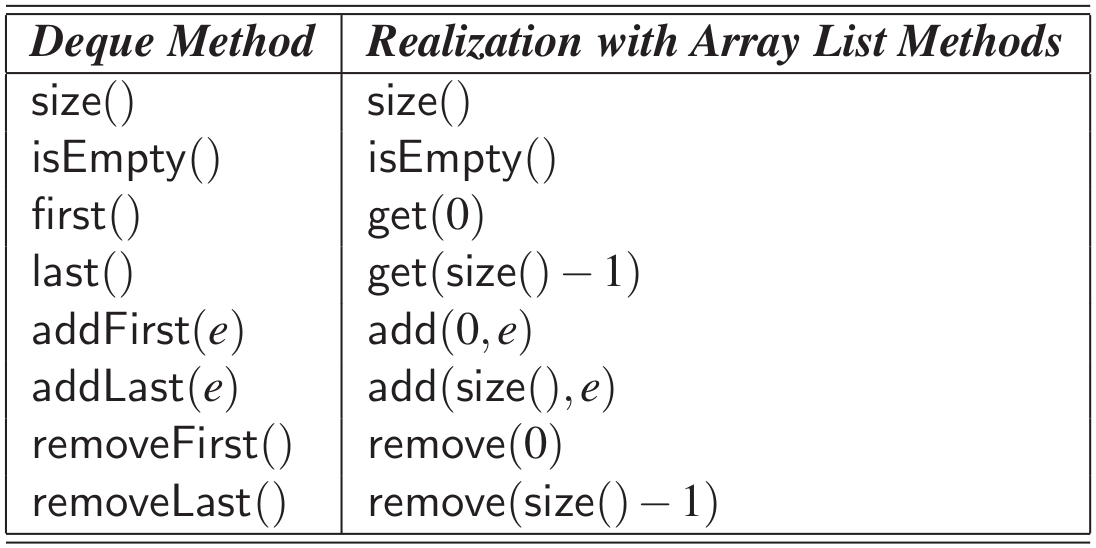
\includegraphics[width=0.6\linewidth]{img/r-7-3}
\end{figure}

\paragraph{Exercício R-7.5:}
O método \texttt{resize} pode ser utilizado para diminuir o vetor.

\begin{lstlisting}[frame=single]
public void trimToSize() {
	if (data.length != size)
		resize(size);
}
\end{lstlisting}

\paragraph{Exercício R-7.7:}
Esta afirmação pode ser verificada experimentalmente. Implemente a estratégia proposta e compare o tempo de execução da versão original e da nova versão. Plote os tempos para verificar o comportamento da curva de resposta.

\paragraph{Exercício R-7.8:}
O tempo de execução para inserir um novo elemento é $n$. Como $n$ elementos são incluídos, o tempo de execução total é $n^2$.

\paragraph{Exercício R-7.9:}
O método \texttt{resize} não pode ser utilizado.

\begin{lstlisting}[frame=single]
public void add(int i, E e) {
	checkIndex(i, size + 1);
	if (size == data.length) {
		E[ ] temp = (E[ ]) new Object[2*data.length];
		for (int k=0; k < i; k++)
			temp[k] = data[k];
		temp[i] = e;
		for (int k=i+1; k < size+1; k++)
			temp[k] = data[k1];
		data=temp;
	} else {
		for (int k=size-1; k >= i; k--)
			data[k+1] = data[k];
		data[i] = i;
	}
	size++;
}
\end{lstlisting}

\paragraph{Exercício R-7.10:}
Modifique o método \texttt{push} de tal forma que ele modifique o tamanho quando necessário.

\paragraph{Exercício R-7.12:}
Conte os passos enquanto percorre a lista até encontrar a posição $p$.

\begin{lstlisting}[frame=single]
public int indexOf(Position<E> p) {
	int count;
	Position<E> walk = first();
	while (walk != p) {
		count++;
		walk = after(walk);
	}
	return count;
}
\end{lstlisting}

\paragraph{Exercício R-7.13:}
Lembre-se de usar o método \texttt{equals} para testar a igualdade.

\begin{lstlisting}[frame=single]
public Position<E> findPosition(E e) {
	Position<E> walk = first( );
	while (walk != null && !e.equals(walk.getElement()))
		walk = after(walk);
	return walk;
}
\end{lstlisting}

\paragraph{Exercício R-7.14:}
Isso causa uma inconsistência interna para ambas as listas, tanto a lista sob a qual a operação é invocada, quanto aquela a que $p$ pertence. Um nodo contendo o novo elemento será ligado na lista à qual $p$ pertence, mas é atualizado o tamanho da lista sob a qual a operação é invocada.

\paragraph{Exercício R-7.15:}
Mapeie cuidadosamente os métodos públicos da interface \texttt{Queue} aos comportamentos concretos da classe \texttt{LinkedPositionalList}.

\paragraph{Exercício R-7.18:}
Lembre-se de utilizar o método \texttt{equals} para testar a igualdade.

\begin{lstlisting}[frame=single]
public boolean contains(Object o) {
	for (int k=0; k < size; k++)
		if (data[k].equals(o))
			return true;
	return false;
}
\end{lstlisting}

\paragraph{Exercício R-7.19:}
Uma boa estratégia consiste em atualizar todas as referências para \texttt{null}.

\begin{lstlisting}[frame=single]
public void clear( ) {
	for (int k=0; k < size; k++)
		data[k] = null;
	size = 0;
}
\end{lstlisting}

\paragraph{Exercício C-7.25:}
Assim como implementado na classe \texttt{ArrayQueue}, é recomendável manter o índice \texttt{f} para a frente da lista e uma variável \texttt{size} para o seu tamanho, que corresponde ao número atual de elementos. O elemento do índice \texttt{k} da lista será encontrado no índice \texttt{(f + k) \% data.length} do vetor de dados. Inserções e remoções podem ser processados tanto no início quanto no fim da estrutura em tempo constante.

\paragraph{Exercício C-7.26:}
Recomenda-se o realinhamento da frente da lista durante a operação \texttt{resize}.

\paragraph{Exercício C-7.35:}
Recomenda-se o realinhamento da frente da fila durante a operação \texttt{resize}.

\paragraph{Exercício P-7.58:}
Exercício de implementação.

\paragraph{Exercício P-7.60:}
Mantenha todas as cartas em uma única lista, e quatro posições para demarcar o inicio dos naipes.

\section{Filas de prioridade}

\paragraph{Exercício 1:}
O primeiro passo consiste em implementar uma classe para a chave. Esta classe armazena os atributos necessários para a ordenação dos passageiros (plano, prioritário e idade). Esta classe deve implementar a interface \texttt{Comparable}, de modo a utilizar o comparador padrão da fila de prioridades. Uma alternativa é criar uma classe comparadora de passageiros e utilizar como comparador da fila de prioridades. Para testar a aplicação, crie uma coleção de passageiros e insira na fila de prioridades. Chame um a um, observando a ordem com a qual os elementos são removidos da estrutura. Imprima a fila em etapas intermediárias, para verificar as diferenças entre utilizar uma estrutura ordenada e uma não ordenada.

\paragraph{Exercício R-9.3:}
$(1, D)$, $(3, J)$, $(4, B)$, $(5, A)$, $(2, H)$, $(6, L)$.

\paragraph{Exercício R-9.4:}
A melhor estrutura de dados para uma simulação de controle de tráfego aéreo é uma fila de prioridades. Esta estrutura permite manipular os instantes de tempo e manter os eventos em ordem, de tal forma que o evento com menor instante de tempo seja facilmente extraído.

\paragraph{Exercício R-9.5:}
Mantenha uma variável adicional que referencie a entrada mínima atual. Isso permite executar a operação \texttt{min} em tempo constante $O(1)$. Note que a operação \texttt{removeMin} continua necessitando tempo linear $O(n)$. Apesar do \texttt{min} atual ser facilmente encontrado e removido, tal método precisa percorrer todos os elementos restantes para identificar o novo mínimo.

\paragraph{Exercício R-9.6:}
Veja a solução anterior.

\paragraph{Exercício R-9.12:}
A resposta está na Seção 9.2.2 de \cite{GoodrichEtAl2014}.

\paragraph{Exercício C-9.25:}
A solução é manter os time stamps nas entradas da fila de prioridades. Mantenha uma variável $m$ inicializada com $0$. Quando executar a operação \texttt{push} com um elemento $e$, chame \texttt{insert(m,\,e)} e decremente $m$. Na operação \texttt{pop}, chame \texttt{remove} e incremente $m$.

\paragraph{Exercício C-9.26:}
A estratégia é similar ao exercício anterior. Mantenha uma variável \texttt{maxKey} inicializada com $0$. Na operação de enfileirar um elemento $e$, chame \texttt{insert(maxKey,\,e)} e incremente \texttt{maxKey}. Na operação de desenfileirar, chame \texttt{removeMin}.

\paragraph{Exercício C-9.27:}
É sempre possível que um novo elemento receba uma chave estritamente menor que a atribuída ao elemento previamente inserido?

\paragraph{Exercício C-9.28:}
Gerencie a estrutura de forma circular.

\section{Mapas}

\paragraph{Exercício 1:}
Exercício de leitura.

\paragraph{Exercício 2:}
Primeiro, você deve criar uma classe para modelar a chave, composta pela nota e pelo preço médio. Crie também uma classe para modelar um restaurante, contendo seu nome, horário de funcionamento e endereço. Crie um mapa para cada uma das quatro categorias. Crie as rotinas de criação de novos restaurantes e exclusão de restaurantes dos mapas. Crie também um método de consulta, dada uma nota e um valor de referência. Questões a serem resolvidas: o que acontece quando dois restaurantes possuem a mesma nota e o mesmo preço médio? Quais alterações precisam ser feitas para as operações de consulta? Como implementar o sistema considerando que um restaurante pode ter mais de uma categoria simultaneamente?

\paragraph{Exercício R-10.1:}
A primeira inserção consome $O(1)$, a segunda consome $O(2)$, e assim por diante. A execução completa dessa operação consome $O(n^2)$.

\paragraph{Exercício R-10.2:}
Basta substituir a lista baseada em vetor pela lista posicional. Para a remoção, pode ser utilizado o método \texttt{remove} da \texttt{PositionalList}.

\paragraph{Exercício R-10.3:}
Para isso, utilize o método \texttt{findIndex}.

\begin{lstlisting}[frame=single]
public boolean containsKey(K key) {
	return (findIndex(key) != -1);
}
\end{lstlisting}

\paragraph{Exercício R-10.18:}
Dado que o mapa seguirá contendo $n$ entradas no final do procedimento, você pode assumir que cada operação \texttt{remove} consome o mesmo tempo assintótico $O(\log n)$. Logo, a complexidade total no pior caso é $O(n \log n)$.

\paragraph{Exercício R-10.19:}
Novamente, podemos utilizar o método \texttt{findIndex}.

\begin{lstlisting}[frame=single]
public boolean containsKey(K key) {
	int j = findIndex(key);
	return (j < table.size( ) && compare(key, table.get(j)) == 0);
}
\end{lstlisting}

\paragraph{Exercício R-10.20:}
Você deve descrever como os métodos \texttt{get} e \texttt{put} devem ser utilizados/adaptados para realizar tal tarefa.

\paragraph{Exercício R-10.21:}
No novo código, o que acontece quando uma chave buscada é igual a \texttt{table.get(mid)}? A nova versão está incorreta. Isso pode ser verificado considerando como exemplo uma chamada de \texttt{findIndex(20, 0, 2)} para uma tabela contendo \texttt{{10, 20, 30}}. Essa chamada deveria retornar o índice $1$, mas o código apresentado retornará o índice $3$. A nova versão computará o índice corretamente alterando a linha $4$ por \texttt{if (compare(key, table.get(mid).getKey()) <= 0)}.

\paragraph{Exercício C-10.33:}
A solução deve fazer uma única chamada ao método \texttt{findIndex}.

\begin{lstlisting}[frame=single]
public V pullAbsent(K key, V value) {
	int j = findIndex(key);
	if (j == -1) {
		table.add(new MapEntry<>(key, value));
		return null;
	} else {
		return table.get(j).getValue( );
	}
}
\end{lstlisting}

\paragraph{Exercício C-10.45:}
Para a solução, cada entrada do mapa deve armazenar seu índice corrente na tabela.

\section{Outras estruturas de dados lineares}

\paragraph{Exercício 1:}
Exercício de implementação.

\paragraph{Exercício 2:}
Exercício de implementação.

\paragraph{Exercício 3:}
Exercício de implementação.


\section{Busca em estruturas lineares}

\paragraph{Exercício 1:}
Você deverá implementar uma classe \texttt{Conta} com os atributos da mesma (agência, número, saldo). Para permitir a busca, essa classe deve implementar a interface \texttt{Comparable}, ou um \texttt{Comparator} deve ser implementado. Uma vez que a coleção de contas esteja armazenada na estrutura, basta utilizar os algoritmos de busca. No caso de uma estrutura ordenada, a inserção deverá ser feita na posição correta, o que possibilita o uso da busca binária. Calcule o tempo de execução de cada operação para diferentes tamanhos das coleções. Plote os resultados para a comparação.

\paragraph{Exercício 2:}
Veja uma possível implementação na Seção 5.1.3 de~\cite{GoodrichEtAl2014}.

\paragraph{Exercício 3:}
Com uma caneta, marque as referências para início e fim da sub-estrutura considerada em cada iteração da busca. Caso essas referências se cruzem, o elemento não foi encontrado. Caso a referência para o meio da lista aponte para o elemento buscado, seu índice é encontrado.

\paragraph{Exercício 4:}
Para implementar essa modificação, você deve parar a busca com sucesso quando o elemento buscado é igual ao elemento analisado. A busca continua se o elemento buscado for menor que o elemento analisado, e pára sem sucesso, caso contrário. No pior caso, o elemento buscado não está na lista e é maior que qualquer elemento dela. Logo, a lista precisa ser totalmente percorrida e a complexidade continua sendo $O(n)$.

\paragraph{Exercício 5:}
Exercício de implementação. Como exemplo, veja a implementação da busca binária na classe \texttt{SortedTableMap}.

\paragraph{Exercício 6:}
Exercício de consulta.

\section{Ordenação de estruturas lineares}

\paragraph{Exercício 1:}
Exercício de pesquisa/leitura.

\paragraph{Exercício 2:}
Crie uma variável para controlar as trocas feitas no vetor.

\begin{lstlisting}[frame=single]
public void sort(int[] array) {
	for(int i = 0; i < array.length; i++) {
		boolean change = false;
		for(int j = 0; j < array.length - (i + 1); j++)
			if(array[j] > array[j + 1]) {
				swap(j, j + 1, array);
				change = true;
			}
		if(!change) return;
	}
}
\end{lstlisting}

\paragraph{Exercício 3:}
Com essa alteração, cada iteração executa uma busca interna em $O(\log n)$. Logo, o algoritmo pode ser implementado com complexidade $O(n \log n)$.

\paragraph{Exercício 4:}
Resultado: a primeira ordenação não é perdida, pois as relações de grandezas se mantém. Teste este comportamento no papel para pequenas matrizes ($2 \times 2$) a fim de verificar seu comportamento. Implemente esta operação.

\paragraph{Exercício 5:}
Para cada aluno, o sistema deverá fazer a leitura das três notas correspondentes, armazenando a média em um vetor de números reais. Após isso, basta aplicar algum algoritmo de ordenação e retornar os últimos $10$ elementos da estrutura.

\paragraph{Exercício 6:}
Ao invés de uma estrutura contendo números reais, deverá ser utilizada uma estrutura para armazenar objetos da classe \texttt{Redacao}. Além disso, alguma estratégia de comparação de nota deverá ser implementada para que a ordenação opere adequadamente.


\bibliographystyle{apalike}
\bibliography{../referencias}

\end{document}